\chapter{Aplicații asemănătoare}

Acest capitol se focusează asupra prezentării unor soluții asemănătoare ca idee sau ca și tehnologie cu proiectul \textbf{Home Smartify}. 

În prezent, există numeroase astfel de platforme, fiind alese cele mai preferate în rândul utilizatorilor care doresc să își adapteze casa după preferințele personale.

\section{Home Assistant}

Home Assistant (Figura 1.1) este o platformă open-source\footnote{\url{https://opensource.com/resources/what-open-source}.} pentru controlul și automatizarea locuințelor smart. Oferind un mediu centralizat pentru gestionarea dispozitivelor și serviciilor, ea suportă peste 1000 de servicii și device-uri diferite pe care le identifică prin scanarea inițială a rețelei de internet la care sunt conectate.

Orice utilizator are asignat o \emph{amprentă digitală}\footnote{\url{https://www.kaspersky.com/resource-center/definitions/what-is-a-digital-footprint}.} care este folosită spre a îl identifica în mediul online. Confidențialitatea constituie unul din punctele forte ale aplicației Home Assistant, astfel că păstrează toate informațiile în domeniul local și evită pe cât posibil comunicarea cu alte servicii din cloud.

Este recomandat ca acesta să fie instalat pe o platformă Raspberry Pi prin folosirea sistemului de operare pus la dispoziție pe website sau poate fi executat într-un \emph{container Docker}\footnote{\url{https://www.docker.com/}.}, metodă similară cu cea implementată în această licență.

\begin{figure}[h]
	\centering
	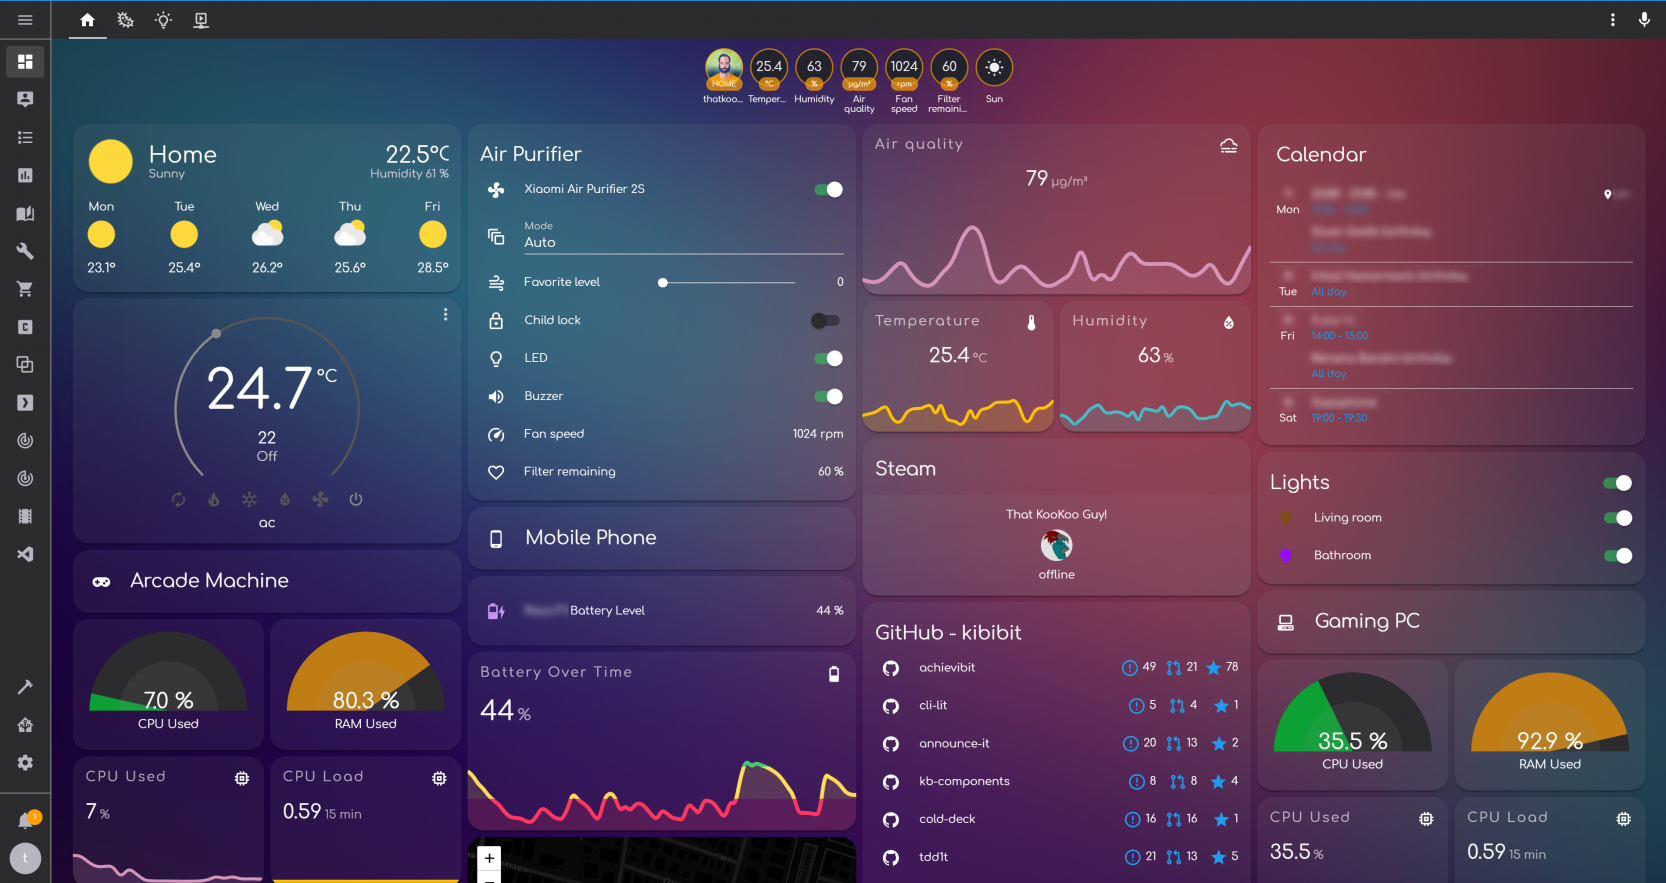
\includegraphics[width=\textwidth]{home_assistant}
	\caption{Interfața meniului principal, temperatură, grafice, consum energie.}\url{https://rbx.dk/w/home-assistant/hvad-er-home-assistant.html}
	\label{fig:home_assistant}
\end{figure}

\section{Apple Home}

Apple este una dintre primele companii care au încercat să integreze controlul casei smart într-o aplicație mobile, lansând HomeKit (Figura 1.2) integrat în IOS 8 care a apărut în septembrie 2014.

Cu suport de peste 100 brand-uri de produse, printre care termostate, prize inteligente, lumini și jaluzele, utilizatorii de Mac, Iphone, Ipad își pot automatiza sarcinile, numite \emph{Scenes}(care pot fi separate pe zone), prin apăsarea unui buton din interfața ușor de înțeles sau pot opta pentru integrarea cu asistentul vocal Siri.

Cristopher Null\footnote{\url{https://www.techhive.com/article/579157/essential-homekit-guide.html}.} de la TechHive afirmă că procesul de instalare este impresionant, dar folosirea acesui program zilnic poate fi \emph{mediocră}, fiind clasificată ultima când vine vorba de control din cauza pierderii semnalului și eșuarea executării task-urilor. Speră ca aplicația să primească update-uri și noi funcționalități, interacțiunea sa cu Apple Home lăsând mult de dorit. Se poate observa numărul de 10 ori mai mic de dispozitive suportate față de Home Assistant, fiind o barieră destul de observabilă atunci când se pune problema extinderii către alte funcționalități.

\begin{figure}[h]
	\centering
	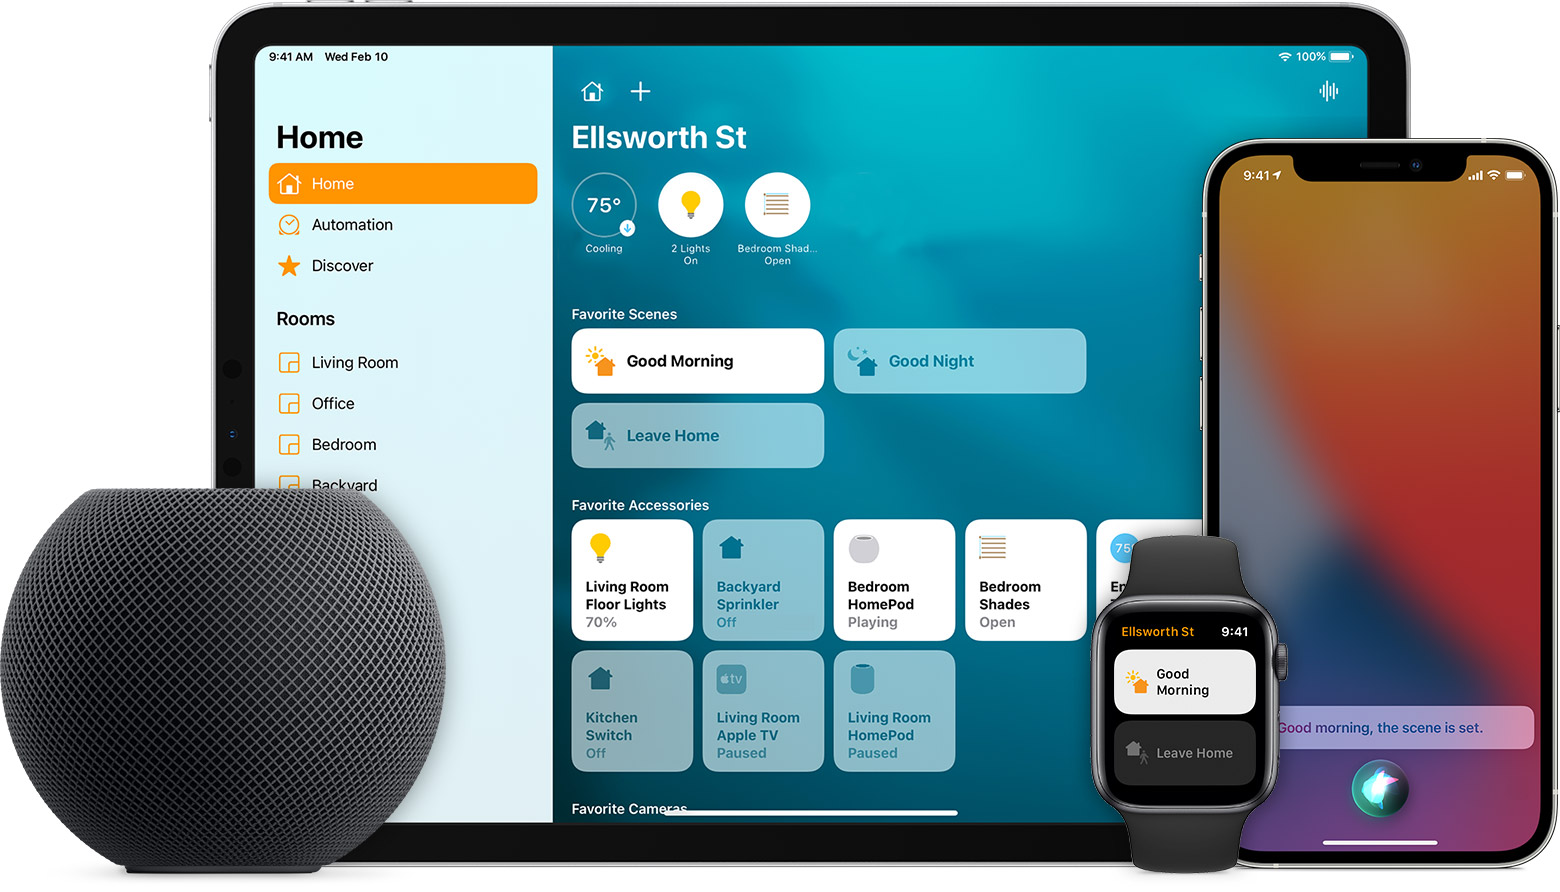
\includegraphics[width=\textwidth]{apple_home}
	\caption{Meniul principal împreună cu dispozitivele ce sunt în control.}\url{https://support.apple.com/en-us/HT208280}
	\label{fig:apple_home}
\end{figure} 


\section{IFTTT}

Fie că dorești să fii notificat pe telefon cu o zi înaintea unui eveniment sau că vrei ca asistentul Google să îți schimbe intensitatea luminilor din garaj, acestea sunt exemplele de bază pe care platforma \emph{IF this then that} (prescurtat \textbf{IFTTT}) (Figura 1.3) le poate realiza.

Acesta este un serviciu ce îți oferă posibilitatea de a conecta aplicații, servicii și dispozitive fără a fi preocupat de programarea lor. Website-ul IFTT și aplicația de telefon te ajută să construiești comenzi (pe care IFTTT obișnuia să le numească \emph{rețete}, acum sunt \emph{applets}) folosind card-uri colorate puternic pentru identificare.

Odată intrat pe pagina de start, se pot vedea applet-urile care sunt conectate cu ajutorul informațiilor de la capătul cardului. Pentru crearea unui astfel de item, trebuie specificat serviciul ce declanșează automatizarea respectivă. Odată ce se întâmplă acel trigger (\emph{if this}), se vor executa acțiunile definite de către utilizator (\emph{then that}). Ex: dacă ai adăugat o melodie nouă într-un playlist pe Spotify, adaug-o și pe Apple Music.


\begin{figure}[h]
	\centering
	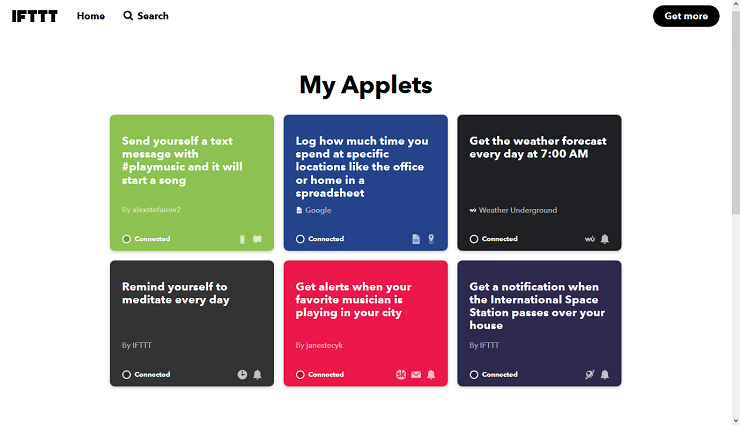
\includegraphics[width=1\textwidth]{IFTTT}
	\caption{Card-urile colorate pentru diferențiere, cu descriere, status și autorul informației.}\url{https://www.pcmag.com/reviews/ifttt}
	\label{fig:ifttt}
\end{figure}

\break
\hfill

\hfill

Prin intermediul ideilor prezentate precedent, putem observa că soluțiile pentru o casă smart sunt din ce în ce mai populare. Este foarte probabil ca un utilizator să dețină dispozitive IoT pe care le poate inter-conecta cu scopul de a obține o utilizare eficientizată a spațiului de lucru.

Soluțiile pentru o casă smart oferă oportunități diverse de a îmbunătăți controlul și automatizarea locuinței. Fiecare platformă are propriile caracteristici și avantaje, iar utilizatorii pot alege în funcție de nevoile și preferințele lor specifice.